% WSCG sample document 
%
% based on Gabriel Zachmann's sample
% http://zach.in.tu-clausthal.de/latex/
%
% modified Apr 2012 to match WSCG Word template
%
\documentclass[twoside,twocolumn,10pt]{article}
%\documentclass[twoside,twocolumn,draft]{article}

%  for debugging
%\tracingall%\tracingonline=0
%\tracingparagraphs
%\tracingpages


%%%%%%%%%%%%%%%%%%%%%%%%%%%%%%%%%%%%%%%%%%%%%%%%%%%%%%%%%%%%%%%%%%%%%%%%%%%%%
%                             Packages

\usepackage{wscg}           % includes a number of other packages (e.g., myalgorithm)
\RequirePackage{ifpdf}
\ifpdf
 \RequirePackage[pdftex]{graphicx}
 \RequirePackage[pdftex]{color}
\else
 \RequirePackage[dvips,draft]{graphicx}
 \RequirePackage[dvips]{color}
\fi
%\usepackage[german,english]{babel}     % default = english
%\usepackage{mypicture}      % loads graphicx.sty, color.sty, eepic.sty
%\usepackage{array}          % better tabular's & arrays, plus math tabular's
%\usepackage{tabularx}      % for selfadjusting p-columns
%\setlength{\extrarowheight}{1ex}   % additional space between rows
%\usepackage{booktabs}      % typographically much better
%\usepackage{mdwlist}        % for compacted lists, and more versatile lists
%\usepackage[intlimits]{amsmath} % more math stuff, see texdoc amsldoc
%\usepackage{mymath}         % own commands, loads amssymb & array.sty
%\usepackage{hyphenat}      % hyphenatable -, /, etc.
%\usepackage{theorem}
%\usepackage[sort&compress]{natbib}% better \cite commands, more flexible
%\usepackage[sort&compress,super]{natbib} % better \cite commands, more flexible
%\newcommand{\citenumfont}[1]{\textit{#1}}


\usepackage{nopageno}       % no page numbers at all; uncomment for final version

\usepackage{subfig}
\usepackage{graphicx}
%%%%%%%%%%%%%%%%%%%%%%%%%%%%%%%%%%%%%%%%%%%%%%%%%%%%%%%%%%%%%%%%%%%%%%%%%%%%%
%                                Title

\title{Automatic morphology: Application on biological images}

\author{
\parbox{0.25\textwidth}{\centering
LE Van Linh\\[1mm]
ITDLU\\
Dalat University\\
Vietnam\\
linhlv@dlu.edu.vn
}
\hspace{0.05\textwidth}
\parbox{0.25\textwidth}{\centering
BEURTON-AIMAR Marie\\[1mm]
LaBRI-CNRS 5800\\
Bordeaux University\\
33400 Talence-F\\
beurton@labri.fr
}
\hspace{0.05\textwidth}
\parbox{0.25\textwidth}{\centering
PARISEY Nicolas\\[1mm]
IGEPP\\
INRA 1349\\
35653 Le Rheu-F\\
nparisey@rennes.inra.fr
}
}

%%%%%%%%%%%%%%%%%%%%%%%%%%%%%%%%%%%%%%%%%%%%%%%%%%%%%%%%%%%%%%%%%%%%%%%%%%%%%
%                          Hyperref


% no hyperlinks
\usepackage{url}
\urlstyle{tt}

% Donald Arsenau's fix for missing kerning of "//" and ":/"
\makeatletter
\def\Uslash{\mathbin{\mathchar`\/}\@ifnextchar{/}{\kern-.15em}{}}
\g@addto@macro\UrlSpecials{\do \/ {\Uslash}}
\def\Ucolon{\mathbin{\mathchar`:}\@ifnextchar{/}{\kern-.1em}{}}
\g@addto@macro\UrlSpecials{\do : {\Ucolon}}
\makeatother





%%%%%%%%%%%%%%%%%%%%%%%%%%%%%%%%%%%%%%%%%%%%%%%%%%%%%%%%%%%%%%%%%%%%%%%%%%%%%
%                              My Commands


%\DeclareMathOperator{\sgn}{sgn}

%\theorembodyfont{\upshape}
%\theoremstyle{break}
%\theoremheaderfont{\bfseries\normalsize}

%\newtheorem{lem}{Lemma}
%\newtheorem{defn}{Definition}



%%%%%%%%%%%%%%%%%%%%%%%%%%%%%%%%%%%%%%%%%%%%%%%%%%%%%%%%%%%%%%%%%%%%%%%%%%%%%
%                                Document


\begin{document}

\twocolumn[{\csname @twocolumnfalse\endcsname

\maketitle  % full width title


\begin{abstract}
\noindent
Morphology is a important characteristics of the biological analysing. Knowing the morphology of an object do not only help us generate the information of the object or re-construct the object but we also classify the objects. Indicating the morphology in biological image is a large field and having many methods from manual methods to semi-automatic or automatically. In the content of this article, we proposed a method to automatic determine the characteristics to define the morphology in biological, specify on beetle. Through segmentation and registration, our method is used to determine the landmarks on the images. The experiment is done with two datasets. The result is evaluated by the coordinates of automatic landmarks and the centroid size of all estimated landmarks.

\end{abstract}

\subsection*{Keywords}
Automatic morphology, landmarks identification, image registration.

\vspace*{1.0\baselineskip}
}]



%%%%%%%%%%%%%%%%%%%%%%%%%%%%%%%%%%%%%%%%%%%%%%%%%%%%%%%%%%%%%%%%%%%%%%%%%%%%%


\section{Introduction}

\copyrightspace

In biology, morphology analysis is widely used to keep the changing information of the organism or detecting the difference information between the organisms. From the result of morphology analysis, we can conclude the evolution of an organism family, or we may classify the organisms. Especially in agriculture, morphology is one of best ways to learn about the variations of the insect on crops. The morphology methods may be divided into the groups by the features which are used by the methods such as shape, structure, color, pattern or size of the object. In the aim to study the potential links between these variations and agricultual ecosystems, a set of 291 beetles has been collected with all the information about the sex, place where they are found and agricultural practices in each field were recorded. For each beetle, the morphometric landmarks has been defined on each part (each insect includes five parts (see figure \ref{figparts})) of the insect by the biologies. Morphometric landmarks are points that can be defined in all speciemns and located precisely. Landmarks are widely used in many biological studies and they are currently included into the classification procedures.\\[0.2cm]
\begin{figure}[h]
\centering
\subfloat[]{\label{figrbox1}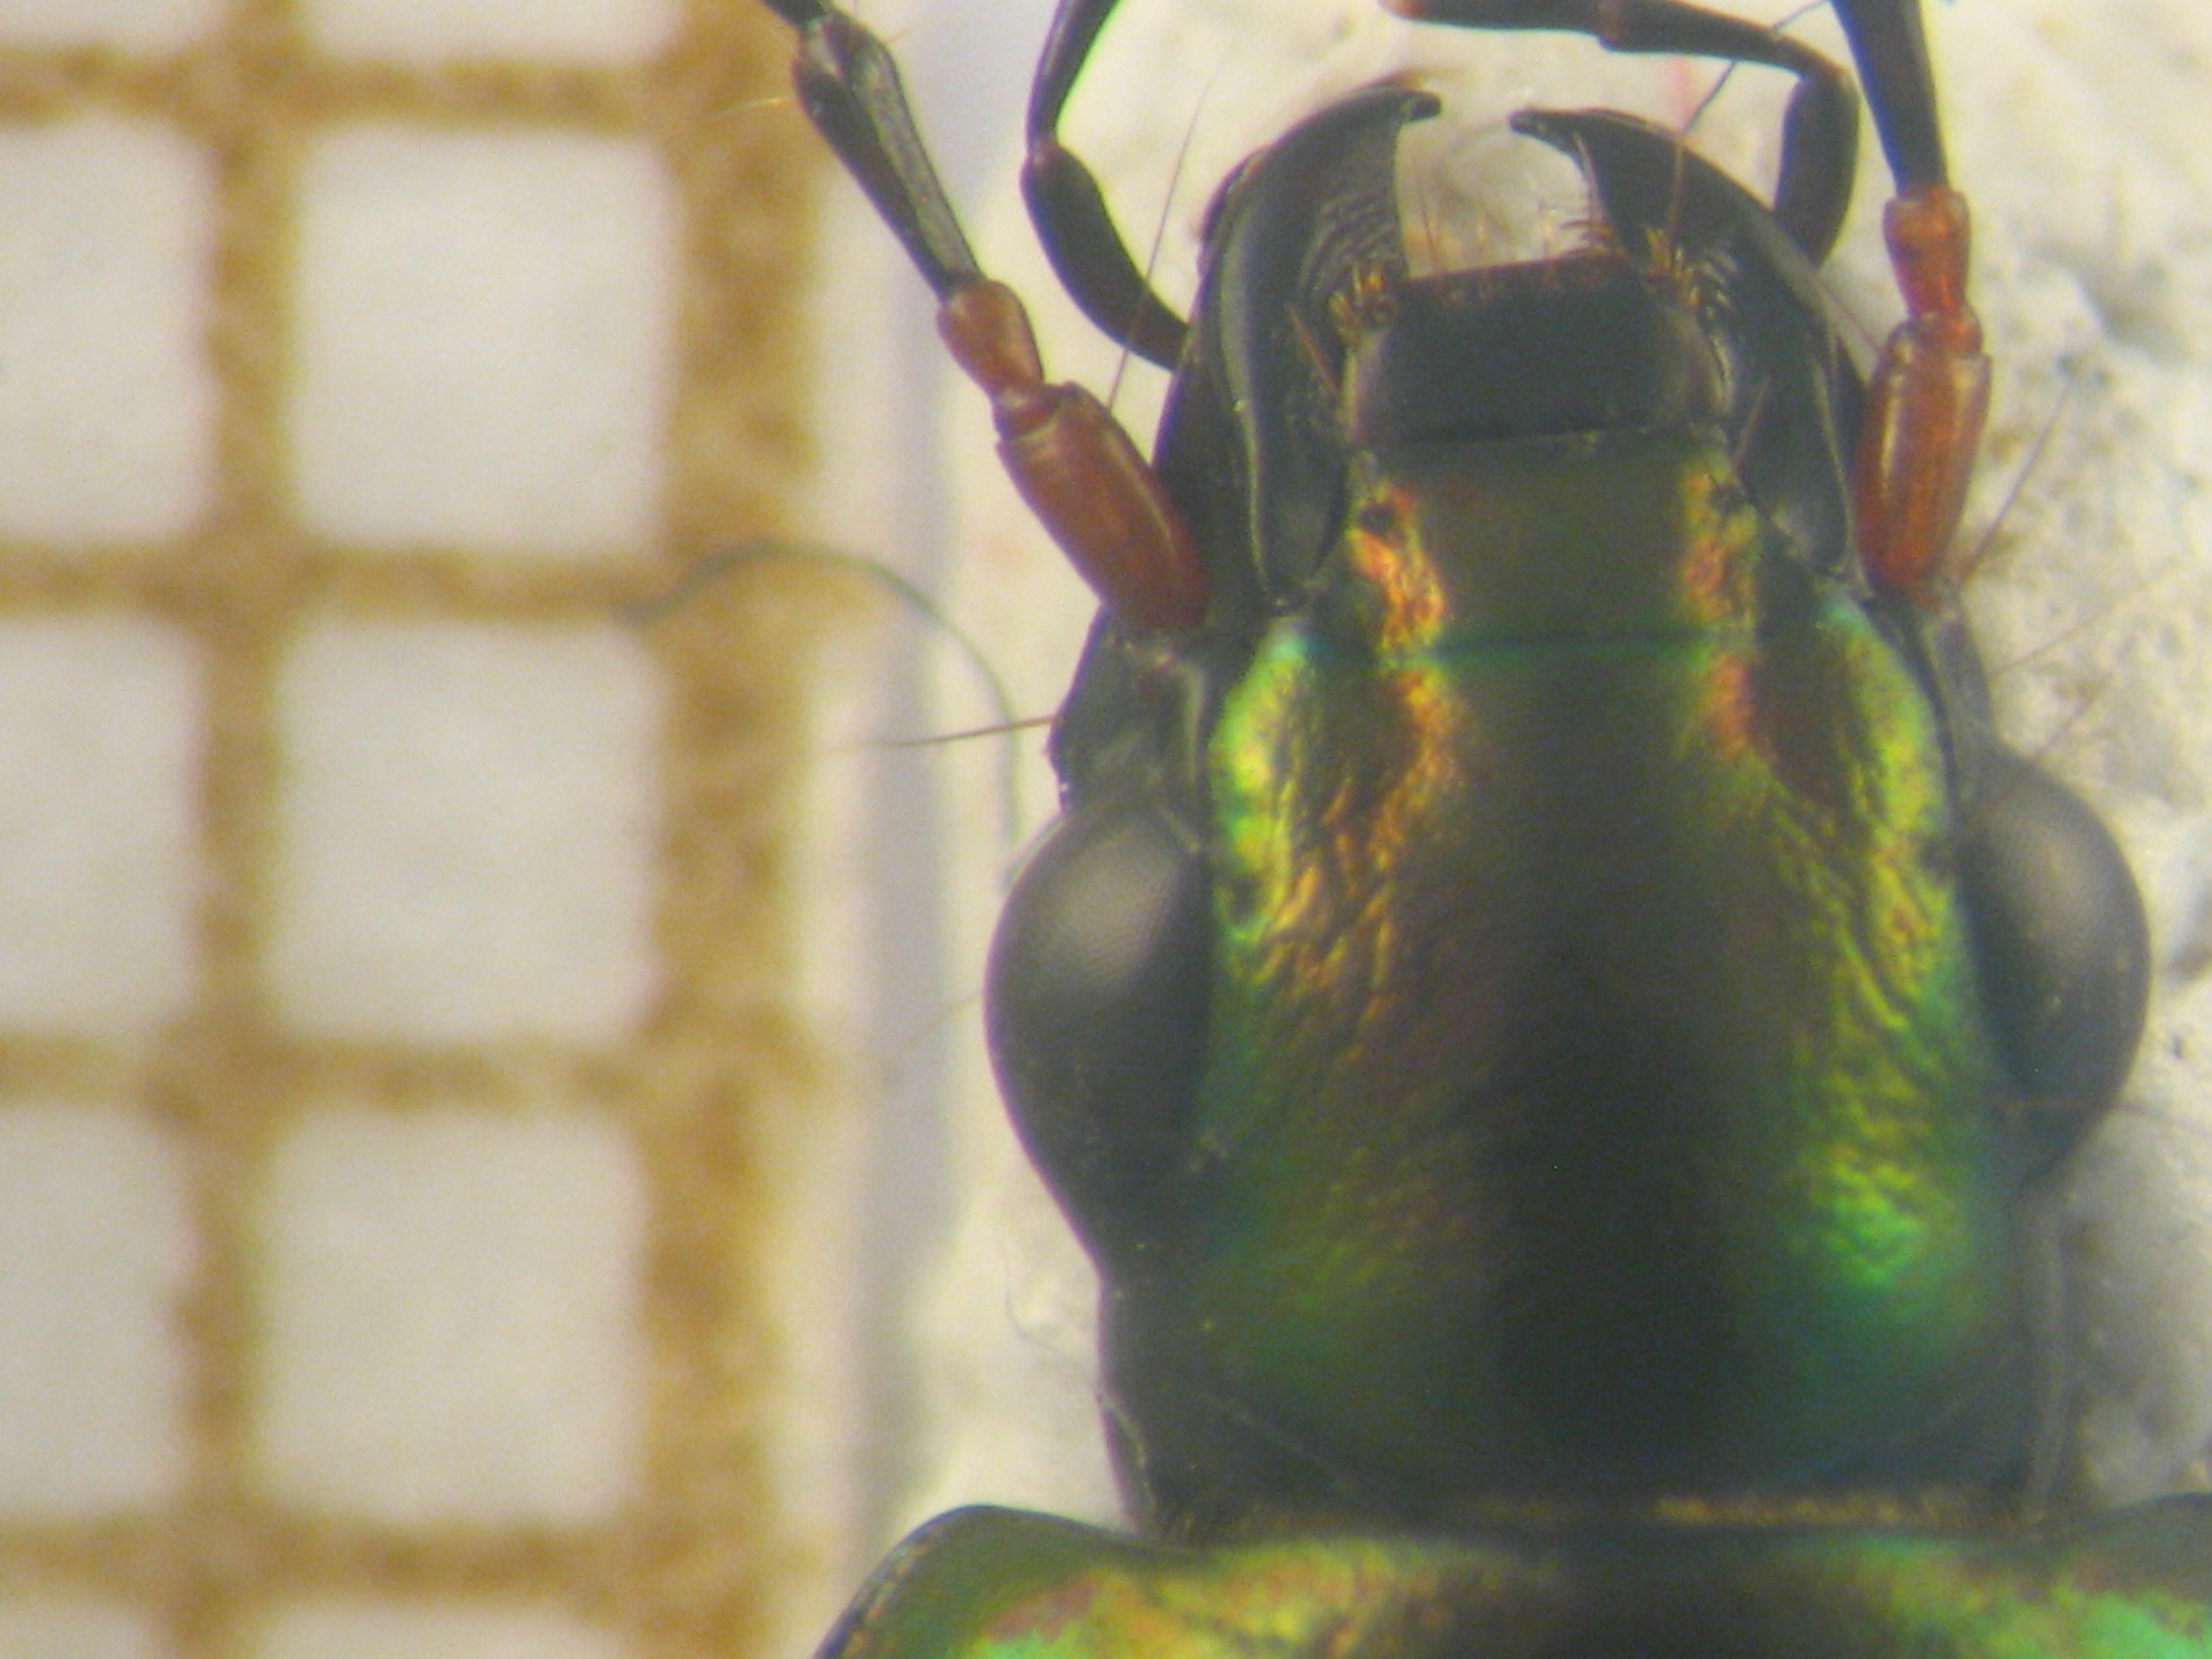
\includegraphics[width=0.22\textwidth]{./images/tete}}~~
\subfloat[]{\label{figrbox2}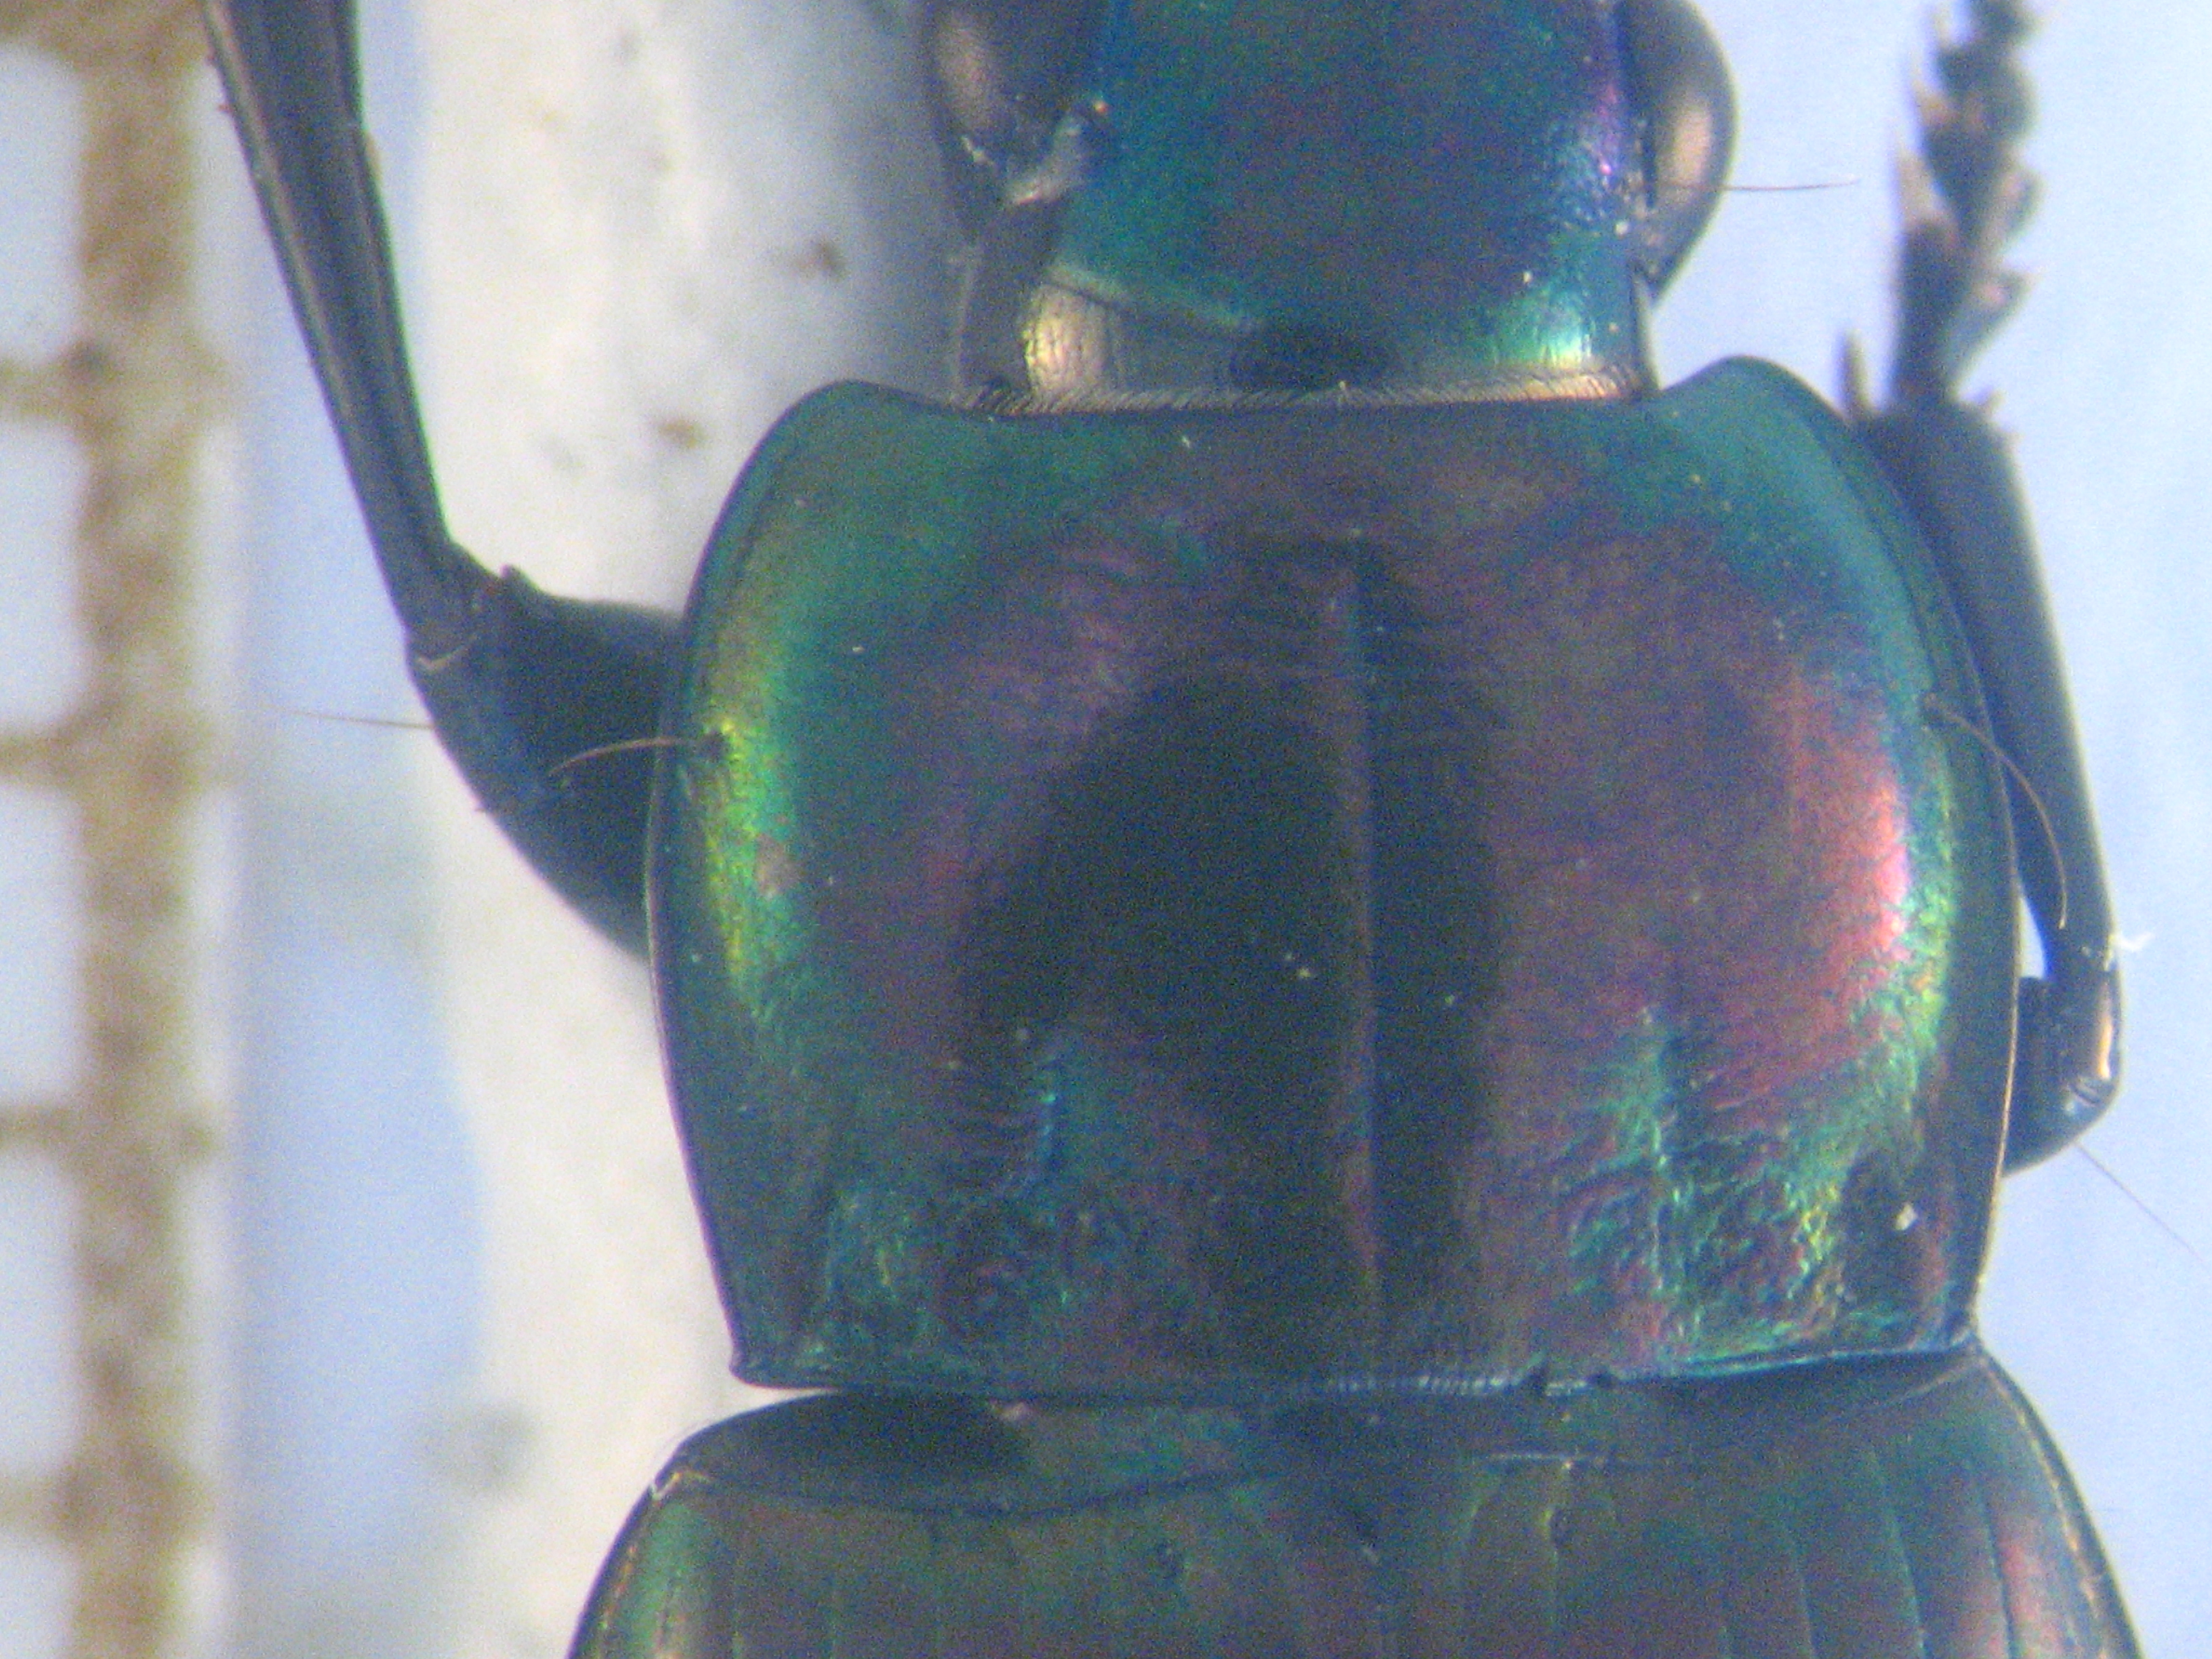
\includegraphics[width=0.22\textwidth]{./images/pronotum}}\\
\subfloat[]{\label{figrbox1}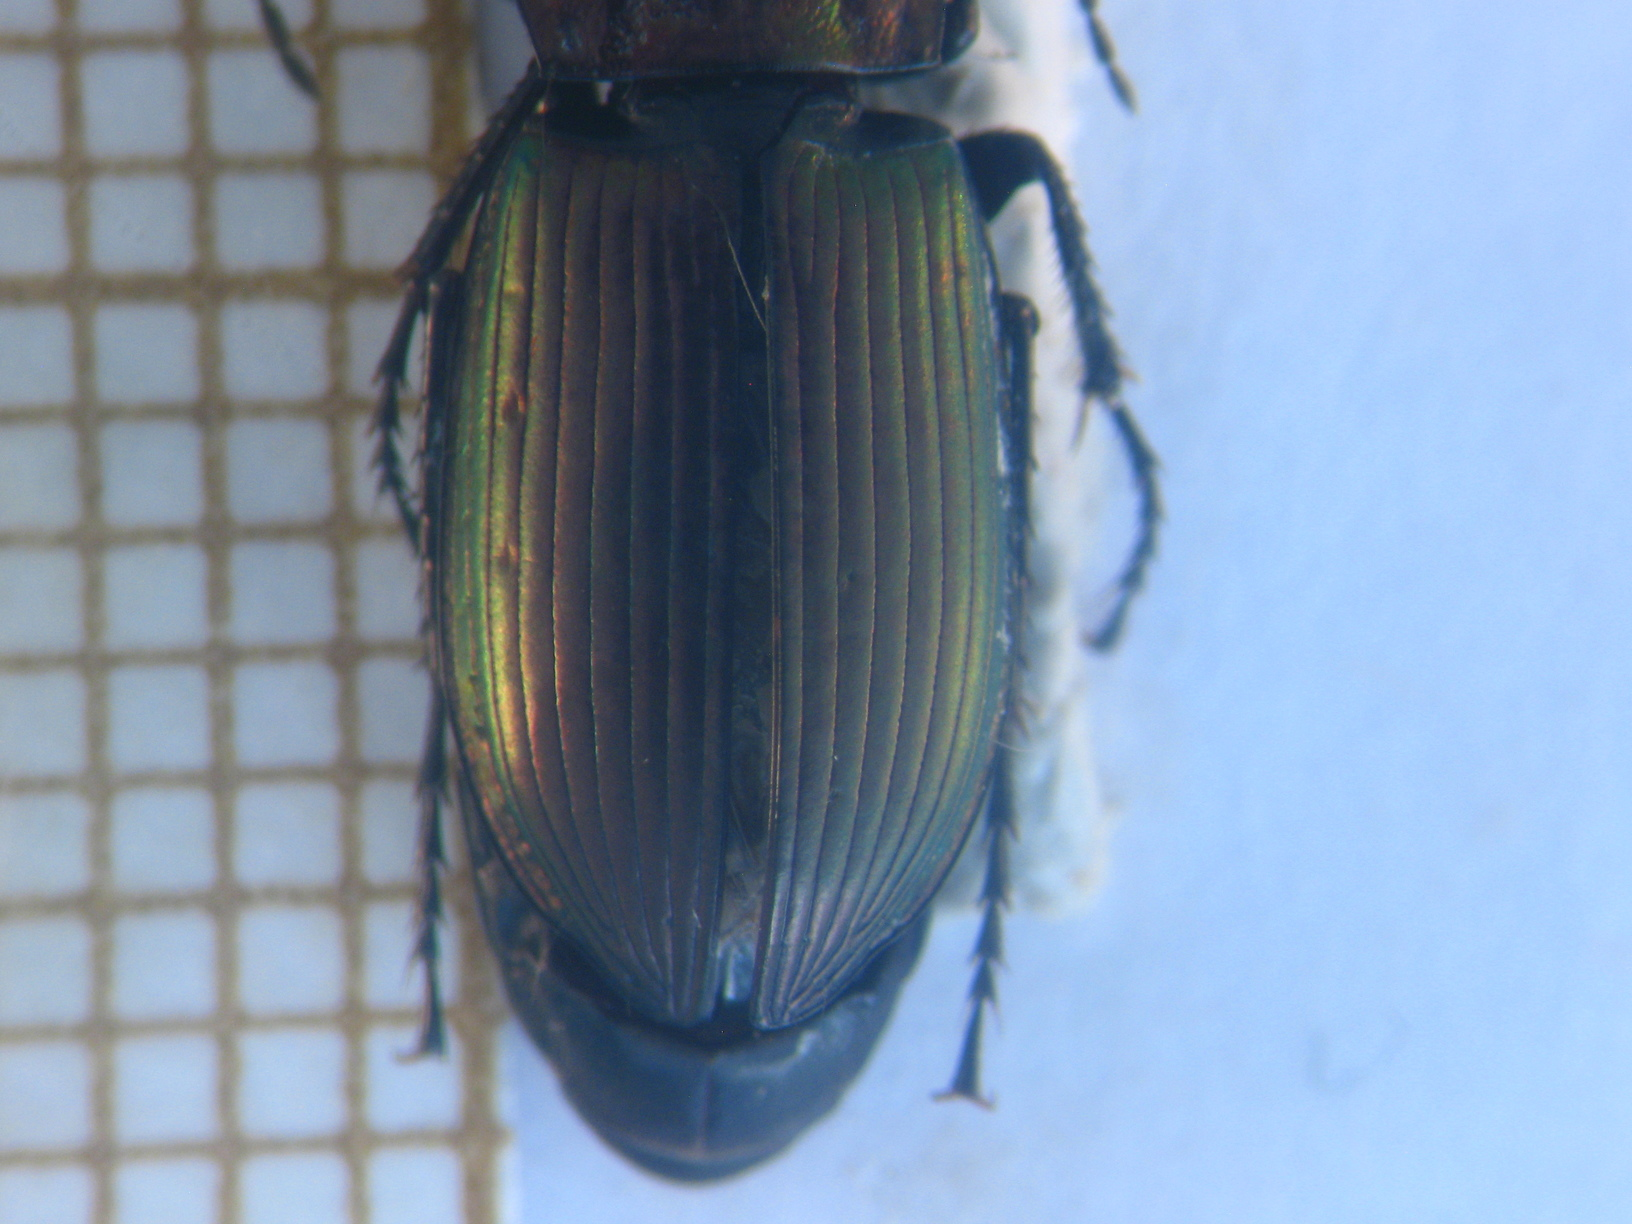
\includegraphics[width=0.22\textwidth]{./images/body}}~~
\subfloat[]{\label{figrbox2}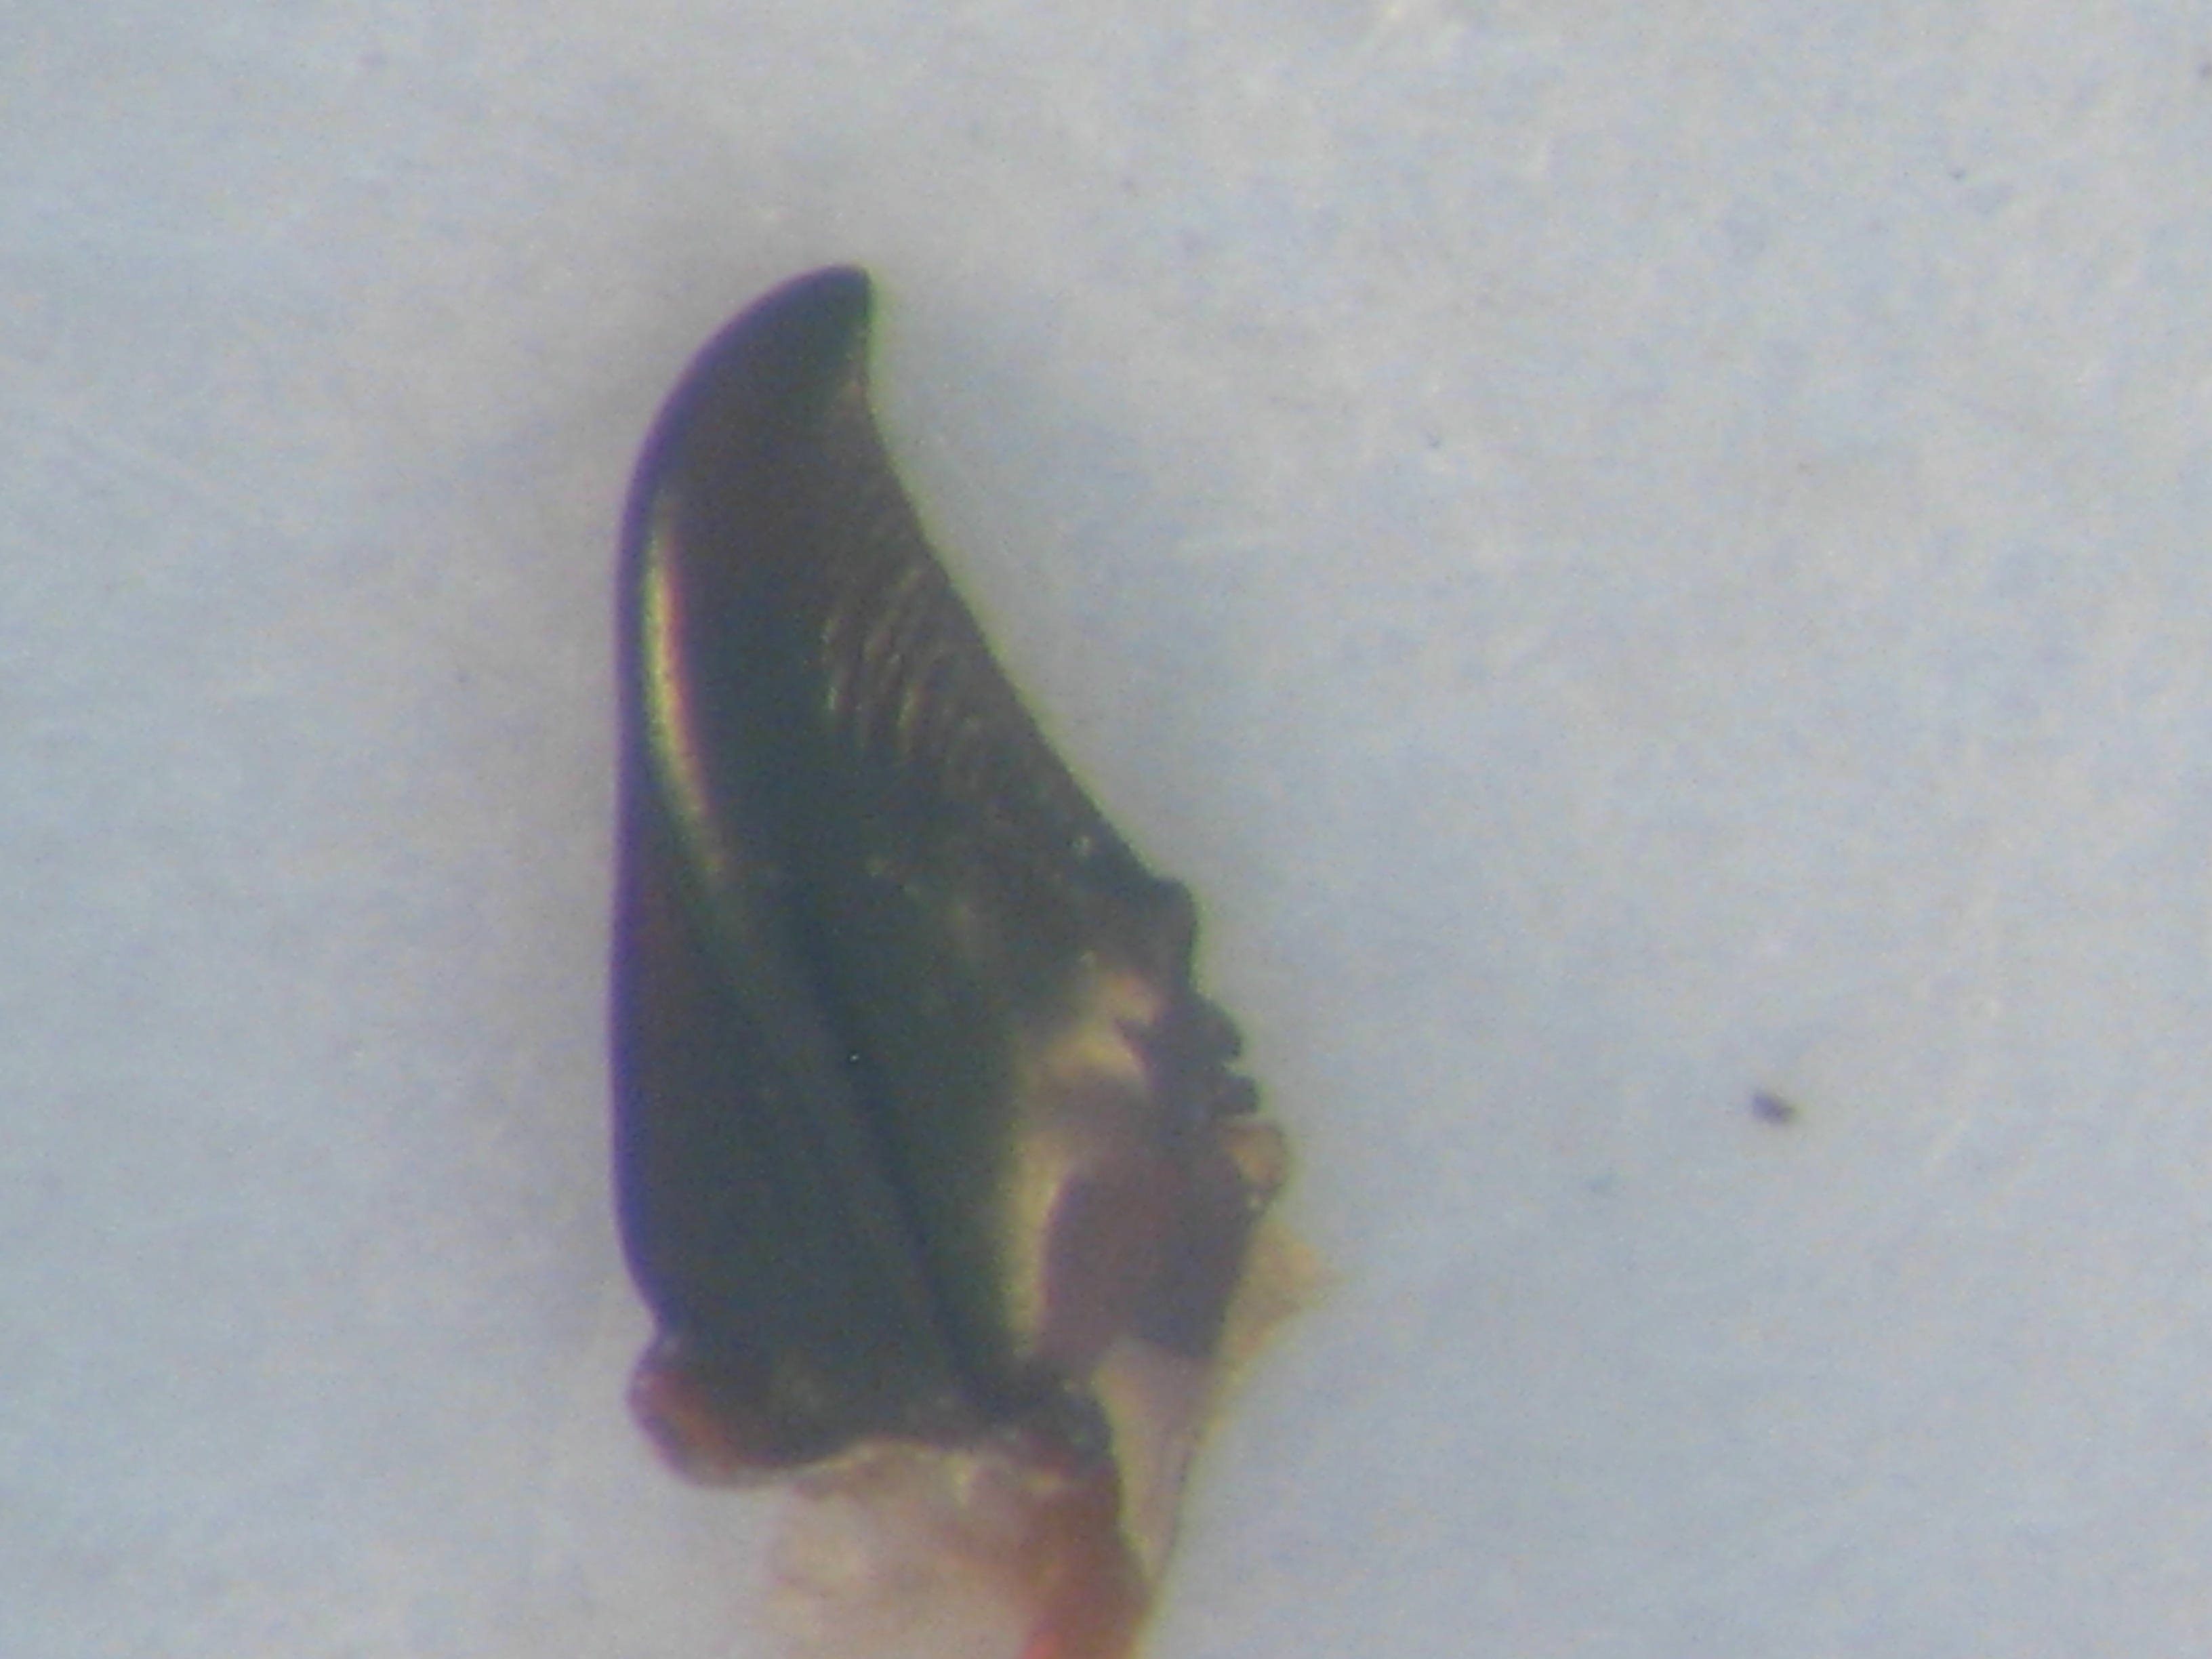
\includegraphics[width=0.22\textwidth]{./images/lm}}\\
\subfloat[]{\label{figrbox1}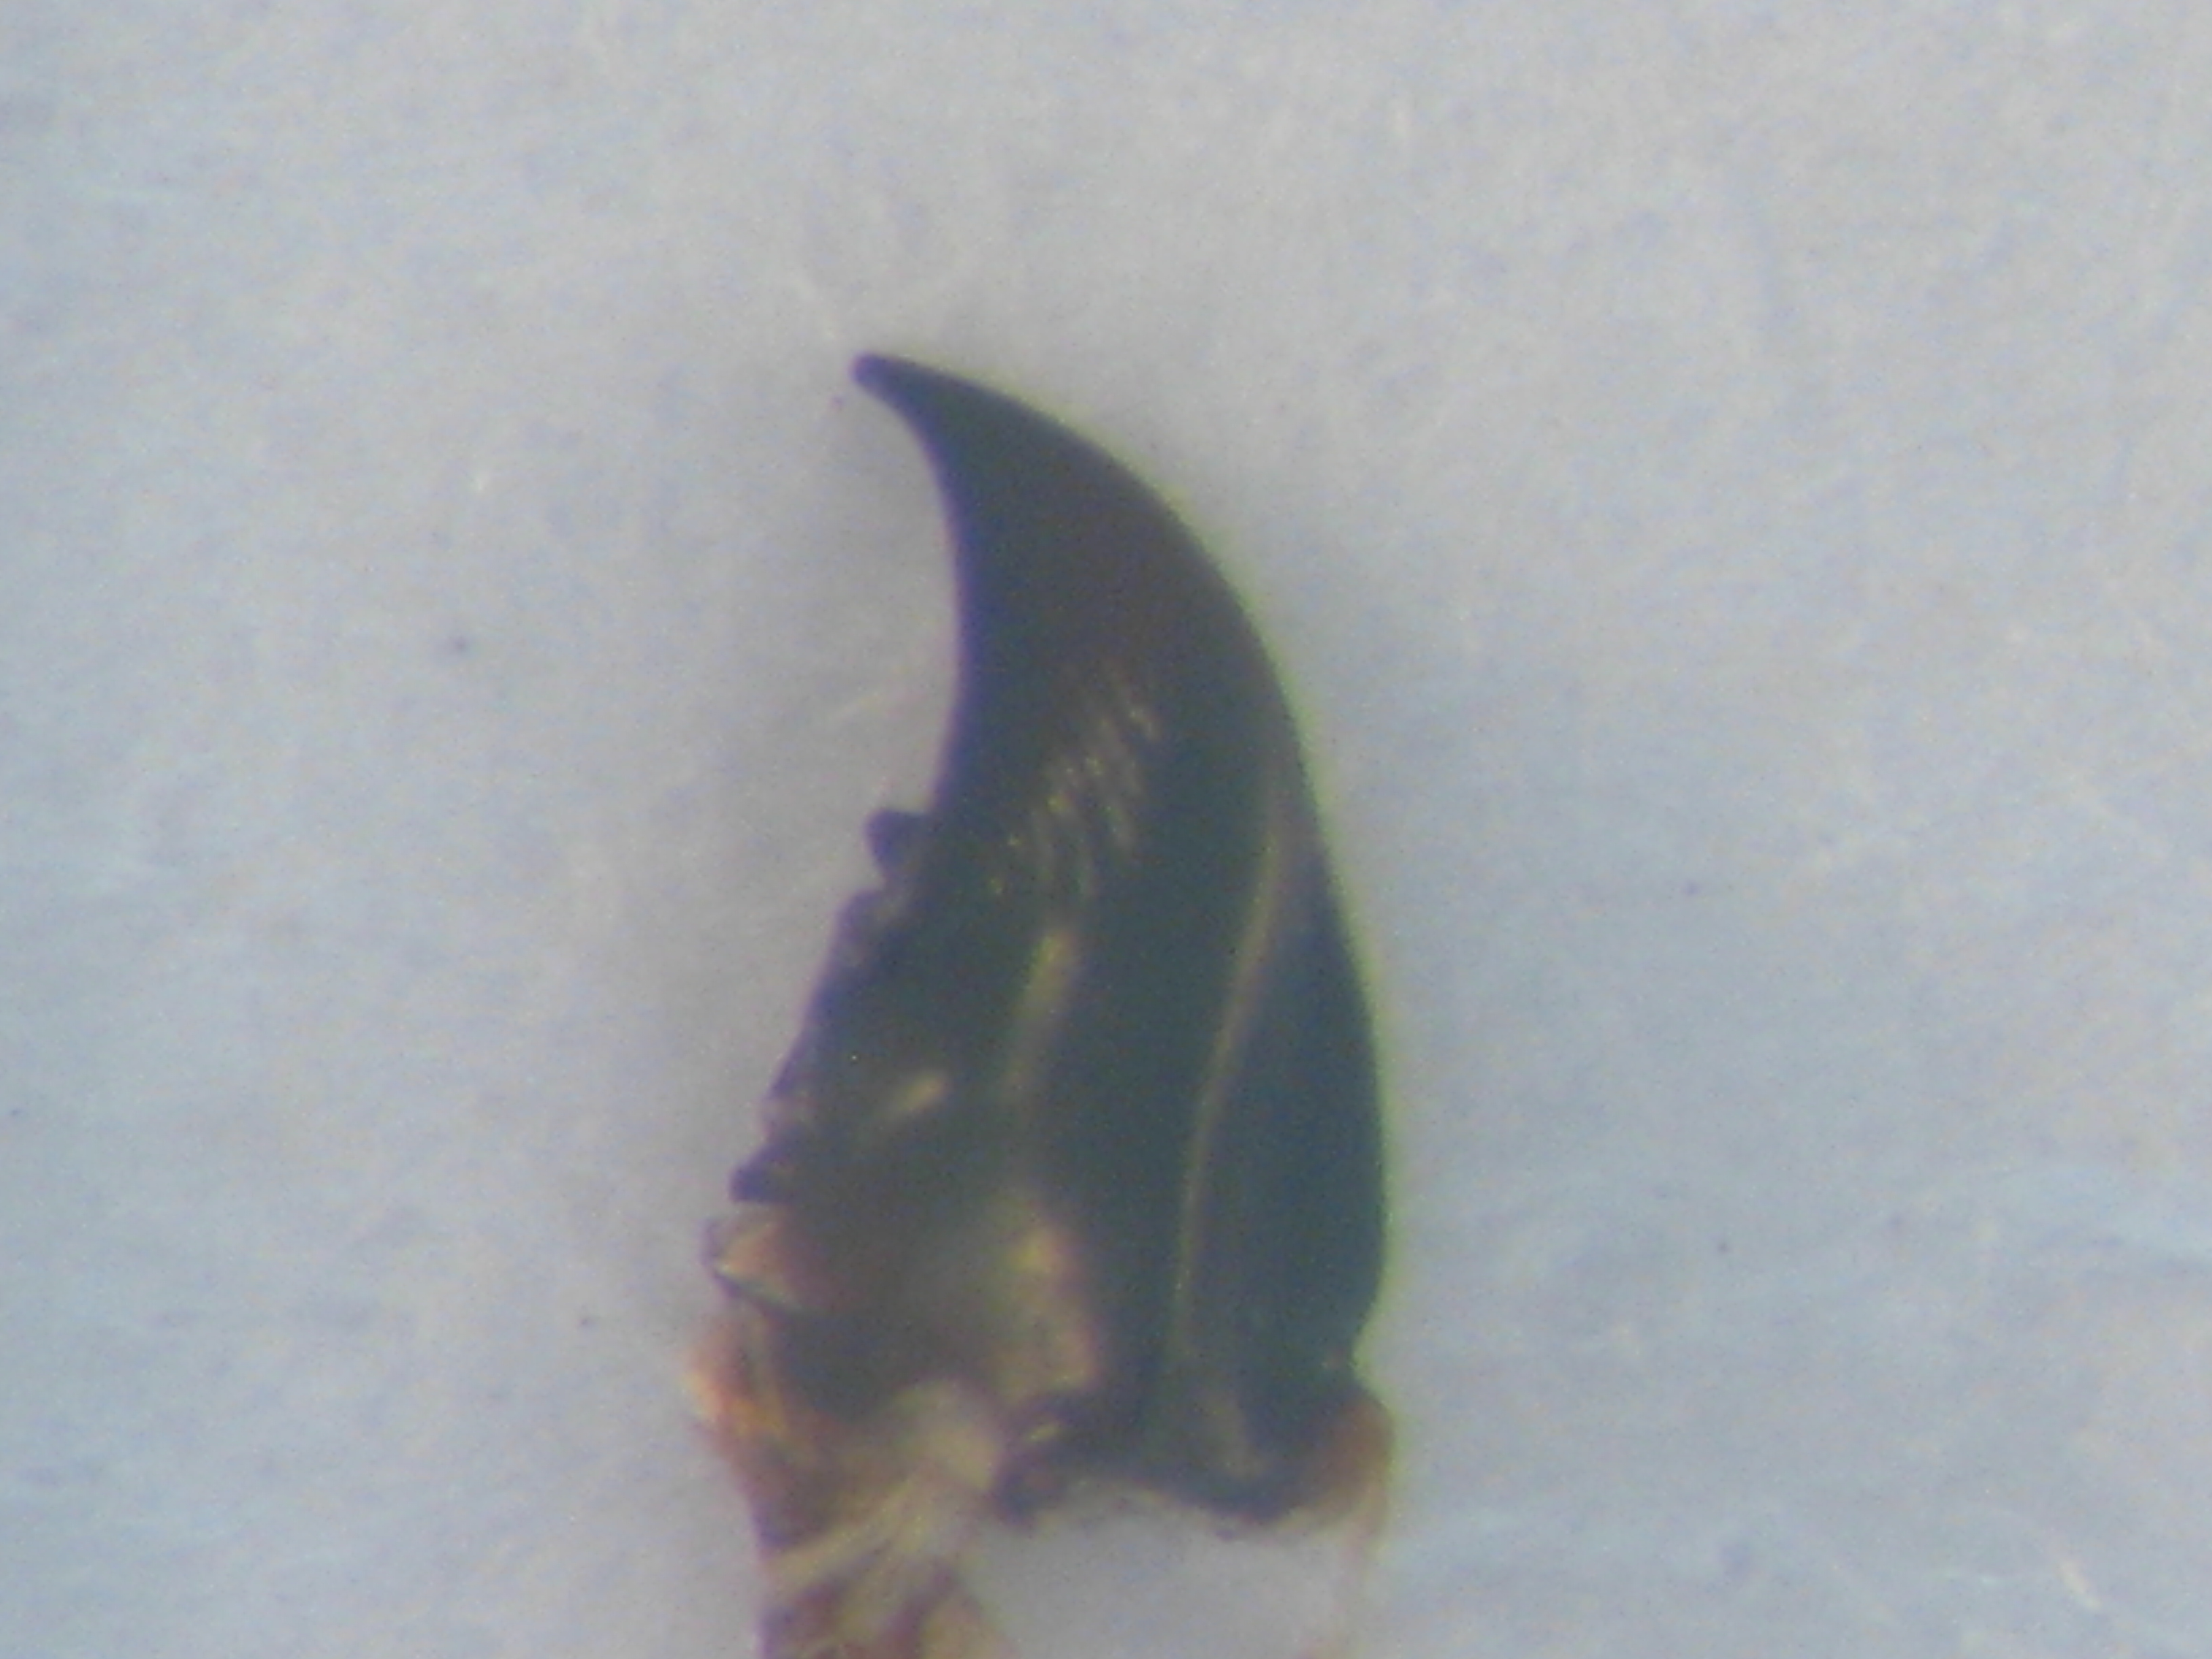
\includegraphics[width=0.22\textwidth]{./images/rm}}
\caption{The parts of beetle: (a) head, (b) pronotum, (c) body, (d,e) left and right mandible}
\label{figparts}
\end{figure}~\\[0.2cm]
In this paper, we focus on a method that can automatic identification of landmarks on 2D images of beetle, specify the mandibles of beetle. The method mainly includes four stages: firstly, we extract the features of the object in the image; secondly, generalizing Hough transform is used to detect the presence between two images; thirdly, the translation and rotation is identified by applying image registration; finally, a refinement of the estimated landmarks is done by cross-correlation.\\[0.2cm]
In section 2, the steps of our methods will be discussed. All experiments and evaluation are described in section 3. Finally, we have some conclusion in the section 4.

\section{Method}
For each image, a set of manual landmarks have been set by biologists corresponding to the morphological points of interest (18 landmarks for each right mandible and 16 landmarks for each left mandible). The automatic procedure to determine the landmarks is based on the segmentation of the image. The presence between two images are indicated by generalizing Hough transform, along with theirs translation and rotation are determine by applying registration. The last step is using cross-correlation to verify the location of estimated landmarks.
\subsection{Image segmentation}
In the methods of image processing, feature extraction is always a important stage. Besides, depending on the nature of the method, the methods are applied before (pre-processing) or after (post-process) extracting the features. In our method, the original Canny alogrithm\cite{canny} is ideal for detect the curves on the image. The ratio between lower threshold and upper threshold which are used in Canny algorithm is 1:3 (lower threshold approximated to 1 times \textit{threshold value} and upper threshold set to 3 times threshold value). This value is evaluated by the experiments. The \textit{threshold value} has been determined by analyzing the image histogram. During appling the Canny alogrithm to detect the curves of object, the gradient direction of each pixel which belongs to the curves is kept for the next step of the method. 
\begin{figure}[h]
\centering
\subfloat[Segmentation result after applying Canny algorithm]{\label{canny1}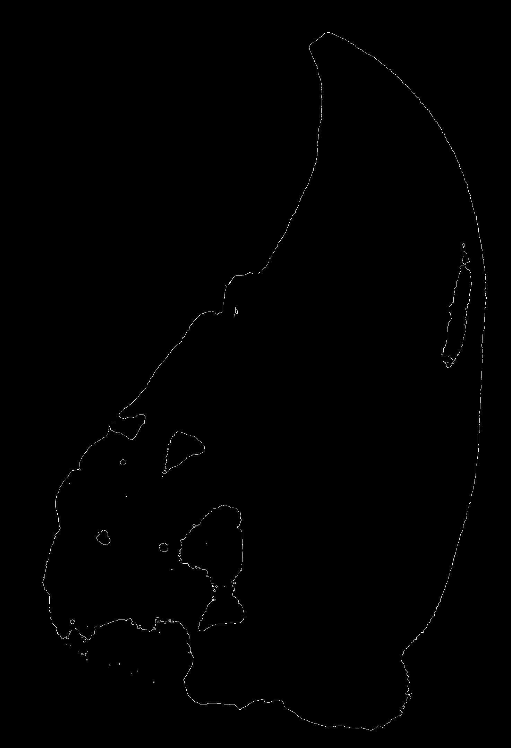
\includegraphics[width=0.2\textwidth]{./images/canny1}}~~
\subfloat[Segmentation result after applying Canny algorithm and post-process]{\label{canny2}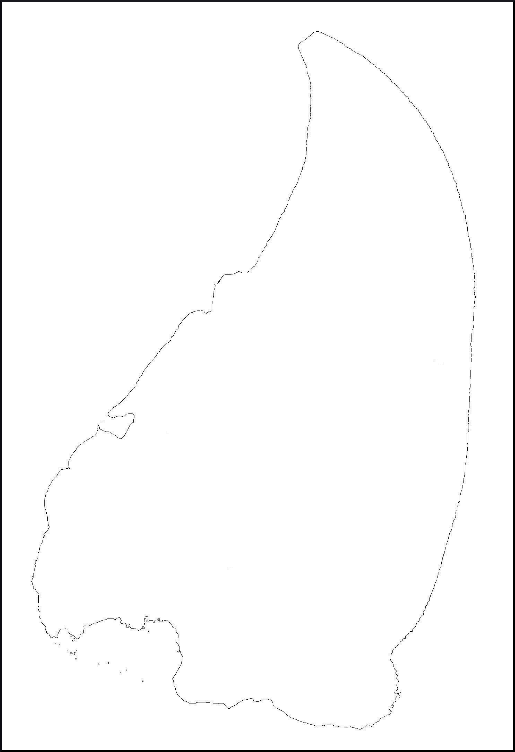
\includegraphics[width=0.2\textwidth]{./images/canny2}}
\caption{The segmentation results of the image}
\label{canny}
\end{figure}~\\[0.2cm]
In this study, the aim of segmentation stage is determined the outer border of the object which can be used to reconstruct the shape of the object as well as provide the best data for next step. The curves from Canny algorithm will be post-processed to remove the unnecessary curves i.e hole inside the border (see figure \ref{canny}). 
\subsection{Generalizing Hough transform}
The generalizing Hought transform (GHT)\cite{Ballard} is a key of this study. With two input images, GHT is used to recognize the similar between two images and estimate the landmarks of an image based on the landmarks of other image. The GHT includes two phases: training and recognition.\\[0.2cm]
\begin{figure}[htb]
    \centering
    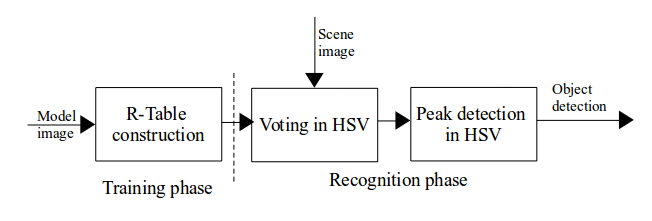
\includegraphics[width=0.5\textwidth]{./images/ghtdiagram}
    \caption{Block diagram of GHT}
    \label{fig:box}
\end{figure}~\\
In the training phase of GHT, model image is used to construct R-table. This is table that contains the polar value of each point in model's curves. A polar coordinate system is initialized in the model image by fixing a reference point and using it as origin. The R-table records the polar coordinate values of all boundary points. The rows of R-table are indexed by the gradient directions of the points on the curves. It means that with a gradient direction can be exists many polar coordinate values.
\begin{table}[htb]
	\centering
	\begin{tabular}{|l|l|l|l|}
	\hline
	Index & Polar values \\
	\hline
	gradient 1 & (r1,l1), (r2,l2),(r3,l3) \\
	\hline
	gradient 2 & (r2,l2),(r4,l4),(r1,l5),... \\
	\hline
	... & ...\\
	\hline
	gradient n & (r1,l1),(r4,l5),(r5,l5),... \\
	\hline
	\end{tabular}
	\caption{An example of R-Table}
\end{table}\\
During the recognition phase, a 2D accumulator is used, called Hough Space Voting (HSV). The axes of HSV express for the information of polar coordinate system. For each curve points on scene image, we try to find a record in R-table that corresponding with the gradient direction of each scene point. The voting will be carried out at all location in HSV that found in R-table. At the end of voting process, if the scene image is identical to the model image, then the cell where have the highest number of votes corresponds to the reference point of the model in the scene image. Besides, the peak value would be equal to the number of curve points of the scene image when the model and scene image match perfectly.\\[0.2cm]
\subsection{Image registration}
Our study is working on 2D image, and the transformation between two images are inevitable. Though, GHT is just hired to detect the presence of model image in scene image. Translation and rotation are determined by applying an alignment method based on the set of boundary points of two images. Firstly, the centroid point of each image is defined by getting mean coordinate of all boundary points. Secondly, a principal axis is indicated for image. This is a connected line from centroid point to a point in list of curve points. For each point in curve, we create a line from centroid point to it, and assume it as an axis. The mean perpendicular distance from the remaining points to axis are calculated. This work is finished for all points on curve, and the principal axis is line that has minimum mean perpendicular distance to other points. The translation is indicated by translation between two centroid points. The rotation is the angle between the principal axis of two images. As well as, the rotation direction is determined by checking each direction.
\begin{figure}[htb]
    \centering
    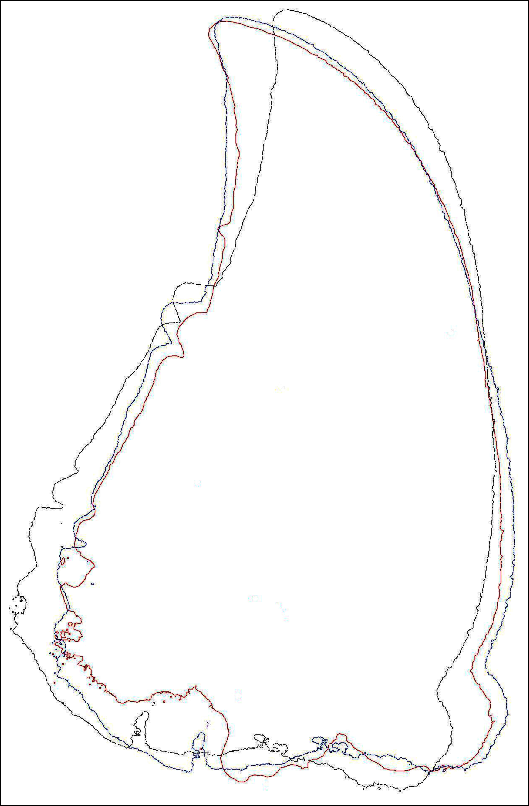
\includegraphics[width=0.2\textwidth]{./images/imreg}
    \caption{A registration result between two images.}
    \label{fig:box}
\end{figure}~\\
At the end of step, the landmarks of scene image are estimated by the manual landmarks of model image. Hence, before estimating the landmarks, a translation and rotation are applied on scene image to match the pose between the scene and the model. The obtained landmarks is computed from the distance from the centroid point to each manual landmarks of the model image.
\subsection{Refinement the estimated landmarks}
The GHT and registration step gave us the estimated coordinate of scene's landmarks. But sometimes the landmarks can be stay at the incorrect location. For this reason, at the end of the method, we apply template matching to verify the location of estimated landmarks. The template matching is done based on the cross-correlation. The equation of cross-correlation is given by equation (\ref{eq:cross-correlation}).
\begin{equation}
\label{eq:cross-correlation}
	R_{ccorr}(x,y) = \sum\limits_{x',y'}[T(x'.y').I(x + x', y + y')]
\end{equation}
Where:
\begin{itemize}
\item T is template which use to slide and find the exist in other image.
\item I is image which we expect to find the template image
\item $(x', y')$ are coordinates in template where we get the value to compute.
\item $(x + x', y + y')$ are coordinates in image where we get the value to compute when template $T$ sliding.
\end{itemize}
For each manual landmark in model, a sub-image \textit{I} with the size \textit{$s_1$} is created; and the corresponding estimated landmark on scene, a template \textit{T} with the size \textit{$s_2$}is created (\textit{$s_1 > s_2$}). The last location of estimated landmarks is the location that has the largest correlation value. Finally, the automatic landmarks are inverted to match with the real location in the scene image (by inverting the transformation).
\begin{figure}[htb]
    \centering
    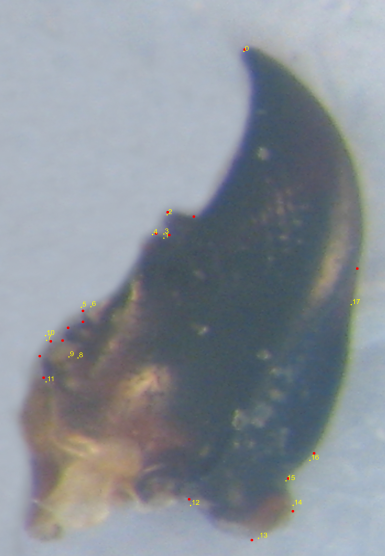
\includegraphics[width=0.3\textwidth]{./images/result}
    \caption{Automatic landmarks after refinement}
    \label{figresult}
\end{figure}~\\
Figure \ref{figresult} show a complete result on one scene mandible with the manual landmarks (red points) and estimated landmarks (yellow points).
\section{Experiments and result}
All the steps in our method are implemented in MAELab\footnote{MAELab is a free software in C++. It can be directly obtained by request the authors.}. Two sets of beetle have been analyzed, right and left mandible. After verifying the quality of the image, it remains 288 usable images for right mandible and 285 images for left mandible. The removed images include the images that do not contain the mandible and the mandible is broken.\\
In all valid images, a set of 18 manual landmarks of right mandible (16 landmarks for left mandible) are indicated by biologists. Along with choosing the centroid size to measure the mandible. This size is obtained by sum of all square distance from each landmarks to the centroid point (see \cite{Webster}).
\begin{figure}[htb]
    \centering
    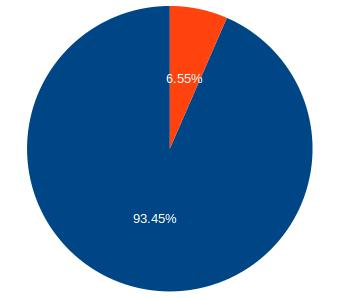
\includegraphics[width=0.5\textwidth]{./images/mdresult}
    \caption{The percentage of correct proportions on right mandibles }
    \label{figmdresult}
\end{figure}~\\
\begin{figure}[htb]
    \centering
    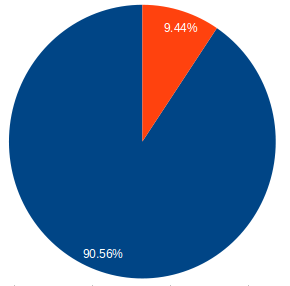
\includegraphics[width=0.5\textwidth]{./images/mgresult}
    \caption{The percentage of correct proportions on left mandibles }
    \label{figmgresult}
\end{figure}~\\
By this way, we have compared the centroid size between manual landmarks and estimated landmarks. We can see in figure \ref{figmdresult} and figure \ref{figmgresult} for all images. The correct proportions of estimated landmarks is 73,35\% for right mandible and 56,99\% for left mandible. In fact, this rate is evaluated by choosing an arbitrary image as model. The object in the image are presented with difference size (scale problem) that our method just consider on translation and rotation between two image. So, the error in computing is easy to understand. However, our method is success in indicating the all landmarks for each image; and the location of the landmarks is considered near with the manual landmarks in some asspect.\\
In a different side, when comparing with our previous study (see in \cite{est}). This method has more advantages for implementation process. The memory to detecting the landmarks, along with the times to execute the process are decreased dramatically.
\section{Conclusion}
Morphometric analysis is a powerful tool in biology in classification the species. Automatic identification the characteristics biology of organism is difficult problem. In the content of this paper, we have begun to design a method to segment the beetle mandibles and to indicate automatically landmarks which have been determined by biologists. Each mandible is segmented by applying Canny algorithm. Using GHT and image registration to estimate the landmarks. Finally, cross-correlation will be applied to refine the location of the estimated landmarks. The first version of this method has been implemented. From now, a next stage of our method is to add the features to have the position of landmarks more precisely.
%-------------------------------------------------------------------------
% example of algorithm typesetting
% to allow this, uncomment line 
% \RequirePackage[noend]{myalgorithm}
% in the wscg.sty file
% and download that package from Gabriel Zachmann's page http://zach.in.tu-clausthal.de/latex/
%
%
%\begin{algorithm}
%\hrule
%  \centering
%\begin{algorithmic}
%    \STMT $d_{l,r} = f_B(P_1), f_B(P_n)$
%    \WHILE{ $|d_l| > \epsilon $ and $|d_r| > \epsilon $ and $l<r$}
%        \STMT $d_x = f_B(P_x)$
%        \IF{ $d_x < 0$ }
%            \STMT $l, r = x, r$
%        \ELSE
%            \STMT $l, r = l, x$
%        \ENDIF
%    \ENDWHILE
%\end{algorithmic}
%\hrule
%\caption{Example of some pseudo-code}
%\label{fg:code}
%\end{algorithm}


%-------------------------------------------------------------------------

\begin{thebibliography}{99}
\label{references}
\bibitem[1]{canny} Canny, John. "A computational approach to edge detection." IEEE Transactions on pattern analysis and machine intelligence 6 (1986): 679-698.
\bibitem[2]{Ballard} Ballard, Dana H. "Generalizing the Hough transform to detect arbitrary shapes." Pattern recognition 13.2 (1981): 111-122.
\bibitem[3]{Webster} Webster, M. A. R. K., and H. DAVID Sheets. "A practical introduction to landmark-based geometric morphometrics." Quantitative Methods in Paleobiology 16 (2010): 168-188.
\bibitem[4]{est} Le Van, L., et al. "Estimating landmarks on 2D images of beetle mandibles."
\end{thebibliography}

%{\bfseries
%Last page should be fully used by text, figures etc. Do not leave empty space, please. 

%Do not lock the PDF -- additional text and info will be inserted, i.e. ISSN/ISBN etc. 
%}


\end{document}
